% https://tex.stackexchange.com/questions/33150/creating-node-shapes?rq=1
\documentclass[border=10pt]{standalone}

\usepackage{tikz}

\makeatletter
\tikzset{arc style/.initial={}}
\pgfdeclareshape{circle with arcs}{
    \inheritsavedanchors[from=circle]
    \inheritanchorborder[from=circle]

    \inheritanchor[from=circle]{center}
    \inheritanchor[from=circle]{south}
    \inheritanchor[from=circle]{west}
    \inheritanchor[from=circle]{north}
    \inheritanchor[from=circle]{east}
    % etc.

    \inheritbackgroundpath[from=circle]

    \beforebackgroundpath{
        % get and set options
        \pgfkeys{/tikz/arc style/.get=\tmp}
        \expandafter\tikzset\expandafter{\tmp}
        \tikz@options

        % get radius length and center coordinates
        \radius \pgf@xa=\pgf@x
        \centerpoint \pgf@xb=\pgf@x \pgf@yb=\pgf@y

        % draw arc starting from north
        \advance\pgf@yb by\pgf@xa
        \pgfpathmoveto{\pgfpoint{\pgf@xb}{\pgf@yb}}
        \pgfpatharc{180}{270}{\pgf@xa}

        % draw arc starting from south
        \advance\pgf@yb by -2\pgf@xa
        \pgfpathmoveto{\pgfpoint{\pgf@xb}{\pgf@yb}}
        \pgfpatharc{0}{90}{\pgf@xa}

        \pgfusepath{draw}
    }
}
\makeatother

\begin{document}
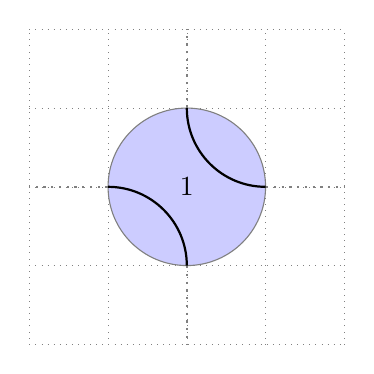
\begin{tikzpicture}
    \draw[help lines, gray, dotted] (-2,-2) grid (2,2);
    \node[
        circle with arcs,
        draw=gray,
        fill=blue!20,
        minimum width=2cm,
        arc style={black,thick}
        ] (c) {1};
    \draw[thick,gray,dotted]
        (c.north) -- +(0,1)
        (c.east)  -- +(1,0)
        (c.south) -- +(0,-1)
        (c.west)  -- +(-1,0);
\end{tikzpicture}
\end{document}